\documentclass[../../main.tex]{subfiles}
\begin{document}
\chapter{Conclusion}
\label{ch:conclusion}

In this chapter, we present a summary and overview of the contributions made in this thesis on \textit{Sign Language Synthesis by a Decreasing Granularity System from AZee}. We outline the research conducted throughout the thesis in Section~\ref{ch:conclusion:summary}. In Section~\ref{ch:conclusion:opensource}, we delve into the open-source contributions, with a particular focus on the AZee-based sign language synthesis toolkit developed as part of this research. In Section~\ref{ch:conclusion:contributions}, we enumerate our specific contributions, and in Section~\ref{ch:conclusion:future}, we explore potential directions for future research that could build on the work presented in this thesis.

\section{Summary}
\label{ch:conclusion:summary}

This thesis explores innovative approaches to synthesizing sign language using a decreasing granularity system based on the AZee framework. The primary objective was to develop a system that could generate sign language sequences that are linguistically accurate and easier to reproduce, addressing a crucial need in accessible communication technologies for the Deaf and Hard of Hearing communities.

In Chapter~\ref{ch:background_work}, we reviewed the foundational work in describing sign languages, and synthesis techniques, particularly focusing on synthesis from AZee. AZee provides a structured way to describe sign language at varying levels of granularity. However, existing methods often struggle to balance linguistic accuracy with ease of synthesis. 

Chapter~\ref{ch:avatar_creation_pose_synthesis} introduced a layered rigging system for signing avatars, emphasizing the importance of rigging in realistic character animation. It presented a procedural rigging system tailored for sign language gestures, focusing on the upper body. The chapter discussed automating site generation using a raycasting algorithm and improving the rigging process with deformation, inverse kinematics (IK), and forward kinematics (FK) layers. It also introduced constraint-based posture optimization and morph constraints. Finally, the chapter evaluated the system’s performance, accuracy, and animation quality, highlighting the potential for future enhancements in sign language avatar animation. 

In Chapter~\ref{ch:multi-track}, the concept of multi-track and non-linear synthesis is introduced to improve sign language avatar animation. The chapter explores how multi-track control mimics natural human motion by preserving the dynamics of simultaneous gestures, facial expressions, and body movements. Non-linear synthesis ensures correct animation sequences and resolves conflicts between overlapping blocks. It discusses converting AZee Synced Scores into multi-track timelines and optimizing with constraint-based approaches. The chapter also highlights the integration of pre-animated blocks and evaluates the improvements in animation quality and flexibility using Blender's non-linear editor.

Chapter~\ref{ch:facial_expressions} presents facial expressions as a critical component in sign language communication, conveying emotional and grammatical information. The chapter introduces a method for synthesizing facial expressions using the AZee framework, focusing on action units (AUs) from the FACS system to create blendshapes for animating signing avatars. It explores face rigging techniques, motion capture, and the generation of motion curves to create dynamic, realistic facial expressions. The chapter evaluates the accuracy of synthesized expressions through subjective and quantitative measures, demonstrating the potential of this approach for improving the realism of signing avatars.

Chapter~\ref{ch:intermediate_blocks}, the generation of intermediate blocks in sign language synthesis is explored to improve the natural flow between signs. By leveraging motion curves and AZee templates, the chapter discusses how transitions between constrained blocks can be enhanced in multi-track representations. It introduces interpolation techniques, such as linear and spline interpolation, and reusable motion templates to create smooth, realistic animations. The chapter evaluates the results of template-based interpolation compared to standard methods, highlighting improvements in naturalness and coherence. It concludes with insights on limitations and potential future improvements in finger articulation and generalization of templates.

Lastly Chapter~\ref{ch:pose_correction} introduces pose correction for sign language synthesis, focusing on improving naturalness and accuracy in sign language avatars. The chapter explores the integration of a pose prior model, trained on a French Sign Language motion capture dataset, to guide the correction process using Variational Autoencoders (VAE). The review covers classical Inverse Kinematics (IK) methods, modern data-driven approaches like Motion Matching and Phase-Functioned Neural Networks (PFNN), and latent space representations like VPoser. The chapter demonstrates how the pose correction system refines generated poses for smoother transitions and more realistic animations, while discussing the challenges and future improvements.

\section{Open Source}
\label{ch:conclusion:opensource}

One of the key contributions of this thesis is the open-source implementation of the synthesizor for AZee. The system extends the original AZee language model and integrates it with a decreasing granularity framework to synthesize signs directly in blender~\ref{fig:azee_animator_interface}.

\begin{figure}[ht]
    \centering
    \includegraphics[width=0.8\textwidth]{images/azee_animator_interface.png}
    \caption{AZee animator interface}
    \label{fig:azee_animator_interface}
\end{figure}

The animator interface allows users to write AZee code in a text editor and visualize the corresponding sign language animations in real-time. For this, the animator loads the AZee compiler as a python module and uses evaluates the generated AZee Scores directly on the avatar. The add-on uses blender's None Linear Editor (NLE) to manage the animation blocks and transitions of the multi-track system. The system also supports facial expressions, intermediate blocks and pose correction.

The blender synthesizor was also integrated with the AZVD~\cite{filhol2024software} editor to generate sign language animations directly on a web interface~\ref{fig:azee_web_interface}.

\begin{figure}[ht]
    \centering
    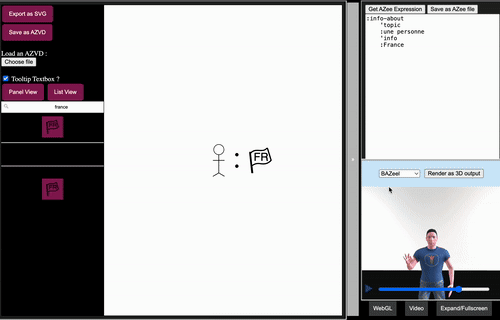
\includegraphics[width=0.8\textwidth]{images/azee_web_interface.png}
    \caption{AZee web renderer interface}
    \label{fig:azee_web_interface}
\end{figure}

The web interface allows users to draw AZee visual descriptions which resolved to AZee Scores and then to animations. For this, the AZee code generated from AZVD in the front-end is sent to the server where an instance of the blender is running headlessly. The synthesizor evaluates the AZee code and returns the animation in video or GLB format to the front-end where it is displayed to the user.

\section{Key Insights}
\label{ch:conclusion:key_insights}

The research conducted in this thesis has yielded several key insights that can inform future work in sign language synthesis and related fields. These insights are summarized below:

\subsection{Granularity}
\label{ch:conclusion:key_insights:granularity}

This thesis highlights the concept of granularity in both sign language representation and synthesis. The term \emph{shortcut} refers to animating linguistic constructs at a higher level of granularity, enabling more natural synthesis while preserving linguistic accuracy, though this comes at the cost of finer control over the animation. Traditional research has typically mapped granularity directly to animations. In contrast, this thesis examines granularity at the posture level, offering a new perspective on sign language synthesis.

Much like how an artist rigs a character with various control points to manage movement, an AZee linguist employs a similar approach to structure sign language discourse. Each control point—whether an IK placement, blendshape, pre-trained pose corrector, or FK rotation—can be seen as a linguistic construct with a certain granularity. This approach allows for the creation of expressive, linguistically accurate animations, offering a more detailed and flexible way to synthesize sign language.

\subsection{Language and Motion}
\label{ch:conclusion:key_insights:language_motion}

The AZee model offers a structured approach to describe sign language, which is crucial because it differs from simply translating sign language to or from a spoken or written language. While an AZee discourse has a one-to-one relationship with its corresponding sign language utterance, the utterance itself can have multiple equivalent translations. Both motion and language are temporal and exist in high-dimensional spaces, but the type of information they carry is different. Body motion operates in a visual space influenced by identity, surroundings, and physical laws, whereas spoken or written language is a human construct, independent of such factors. This distinction doesn't apply to sign languages, as their motion space is tied to their linguistic structure. Thus. while a common \emph{space} between an English sentence and the motion of its sign language translation is unlikely, AZee can provide such a space between sign language descriptions and the motion they represent. This uniqueness is what makes the problem of sign language synthesis different from other newer generative translation techniques.

\section{Future Directions}
\label{ch:conclusion:future}

While the contributions of this thesis mark a progress in sign language synthesis, several avenues for future research remain open. Below, we outline potential research topics that could extend the work presented in this thesis.

\subsection{Enhancing the Decreasing Granularity Model}
\label{ch:conclusion:future:granularity}

\begin{itemize}
    \item \textbf{Dynamic Granularity Adjustment:} Future research could explore methods for dynamically adjusting the level of granularity based on the context or user preferences. This would enable more personalized and adaptive sign language synthesis.
    
    \item \textbf{Integration with Neural Networks:} Incorporating deep learning techniques, such as neural networks, could enhance the model’s ability to generalize across different sign languages and dialects. This integration could also improve the synthesis of signs that involve complex or subtle movements.
\end{itemize}

\subsection{Expanding AZee Framework Capabilities}
\label{ch:conclusion:future:azee}

\begin{itemize}
    \item \textbf{Support for Additional Sign Languages:} While the current system supports a range of sign languages, expanding its capabilities to include more languages and regional dialects would increase its applicability and impact.
    
    \item \textbf{Multimodal Integration:} Combining the sign language synthesis system with other modalities, such as facial expressions and body posture, could lead to a more comprehensive and natural representation of signed communication.
\end{itemize}

\subsection{Real-Time Sign Language Synthesis}
\label{ch:conclusion:future:realtime}

\begin{itemize}
    \item \textbf{Optimization for Low-Latency Environments:} Future research should focus on optimizing the system for real-time applications, such as live interpretation services. This would involve reducing computational load while maintaining the quality of the synthesized signs.
    
    \item \textbf{User-Centered Evaluation:} Conducting extensive user studies to evaluate the system’s performance in real-world scenarios would provide valuable insights for further refinement and development.
\end{itemize}

\subsection{Interdisciplinary Research}
\label{ch:conclusion:future:interdisciplinary}

\begin{itemize}
    \item \textbf{Collaboration with Linguists and Sign Language Experts:} Continued collaboration with linguists and native signers will be crucial for refining the linguistic accuracy and expressiveness of the synthesized signs. This interdisciplinary approach will help ensure that the technology remains aligned with the needs and preferences of the Deaf and Hard of Hearing communities.
    
    \item \textbf{Ethical Considerations:} As sign language synthesis technology evolves, it is important to address ethical considerations, such as ensuring accessibility and avoiding the misrepresentation of signed communication. Future research should incorporate these considerations into the design and deployment of sign language technologies.
\end{itemize}

\subsection{More qualitative evaluation}
\label{ch:conclusion:future:evaluation}

\begin{itemize}
    \item \textbf{Collaboration with Linguists and Sign Language Experts:} Continued collaboration with linguists and native signers will be crucial for refining the linguistic accuracy and expressiveness of the synthesized signs. This interdisciplinary approach will help ensure that the technology remains aligned with the needs and preferences of the Deaf and Hard of Hearing communities.
    
    \item \textbf{Ethical Considerations:} As sign language synthesis technology evolves, it is important to address ethical considerations, such as ensuring accessibility and avoiding the misrepresentation of signed communication. Future research should incorporate these considerations into the design and deployment of sign language technologies.
\end{itemize}


In conclusion, this thesis has laid a strong foundation for the development of advanced sign language synthesis systems. By building on the work presented here, future research has the potential to further enhance the accessibility and effectiveness of communication technologies for the Deaf and Hard of Hearing communities.


\end{document}